\documentclass[11pt,a4paper]{article}
\usepackage[a4paper, total={7in, 10.25in}]{geometry}


\usepackage{color}
\usepackage{graphicx}
\usepackage{wrapfig}
\usepackage{fancyhdr}
\usepackage{tocloft}
\usepackage{multicol}
\usepackage{hyperref}
\usepackage{tabularx}
\usepackage{array}
\usepackage[export]{adjustbox}
\usepackage{listings}
\usepackage{xcolor}
    \definecolor{codegreen}{rgb}{0,0.6,0}
    \definecolor{codegray}{rgb}{0.5,0.5,0.5}
    \definecolor{codepurple}{rgb}{0.58,0,0.82}
    \definecolor{backcolour}{rgb}{1,1,1}

    \lstdefinestyle{mystyle}{
        backgroundcolor=\color{backcolour},   
        commentstyle=\color{codegreen},
        keywordstyle=\color{magenta},
        numberstyle=\tiny\color{codegray},
        stringstyle=\color{codepurple},
        basicstyle=\ttfamily\footnotesize,
        breakatwhitespace=false,         
        breaklines=true,                 
        captionpos=b,                    
        keepspaces=false,                 
        numbers=left,                    
        numbersep=5pt,                  
        showspaces=false,                
        showstringspaces=false,
        showtabs=false,                  
        tabsize=2
    }



\renewcommand{\cftsecleader}{\cftdotfill{\cftdotsep}}
\graphicspath{ {./images/} }
\hypersetup{
    colorlinks=true,
    linkcolor=blue,
    citecolor=black,
    filecolor=magenta,      
    urlcolor=cyan,
    pdftitle={Overleaf Example},
    pdfpagemode=FullScreen,
    }
\pagestyle{fancy}
\setlength{\headheight}{18pt}
\fancyhead[L]{\textit{EN3551 Digital Signal Processing : Assignment 02}}
\fancyfoot[L]{\textit{Department of Electronic and Telecommunication \\University of Moratuwa}}

\title{DEPARTMENT OF ELECTRONIC AND TELECOMMUNICATION
UNIVERSITY OF MORATUWA

\vspace{10pt}

{\large{\textsc{EN3551 Digital Signal Processing}}}

{\textsf{This is offered as a "EN3551 Digital Signal Processing" module's partial completion.}}

\vspace{30pt}

\includegraphics[scale=1.20]{images/University_of_Moratuwa_logo.png}

{\textsf{\textbf{Assignment 02 : Application of 2D-DCT for Image Compression}}}}


\author{200686J : Vishagar A.}

\date{$7^{th}$ of October, 2023}

\begin{document}

\maketitle

\newpage

\begin{abstract}
    \textit{This report deals with the explanation of the solutions for the given questions in the assignment 02 of the EN3551 module. The solutions are explained in a way that it is easy to understand and follow. The solutions are explained with the help of the code snippets and the results. We are mainly focussed on some real world problems like "Application of 2D-DCT for Image Compression". \textbf{And I have used \underline{python} as the programming language to find the solutions for the given problems.}}    
\end{abstract}    

\vspace{50pt}
\tableofcontents


\newpage

\twocolumn

\section{Introduction}

In this assignmet, we are mainly focussed on a real world problem, \textbf{Image Compression} and we need to apply the 2D-DCT for the given image. And we need to find the compression ratio, percentage of zero and the PSNR value for the given images. 

\section{Dataset}

The provided dataset contains \textbf{.mat} files of a image. We need to extract the necessary image data from the .mat file and use it for the further processing. I have assigned to use 3 images from the provided dataset and one image as per my wish.

\section{Methadology}

\subsection{Extracting and Preparing the Data}

As I mentioned earlier, we need to import the required .mat file and extract the image data from the .mat file using the relevant key name. Then if we wish we can visualize and see the imported image.
\\\\
Then after importing the necessary image data, image array was divided in to blocks in a size of 8x8. And meanwhile as we are dealing with negative integer values also, I converted the default image data format from \textbf{np.uint8} to \textbf{np.int16}.


\subsection{Implementation of DCT}

Then after converting into blocks for better results the image data range was converted from \textbf{0 to 255} to \textbf{-128 to 127} , by subtracting 128 from each entry of the image matrix. 
\\
\\
Then for each blocks which we have divided earlier, we need to apply the 2D-DCT. For that I have used the \textbf{dctn() function }  in the \textbf{numpy} library.
\\\\
And then the DCT coefficients were quantized using the given quantization matrix. Standard quantization matrix was given for a quality factor of 50 \% and for the other factors the same matrix was multiplied by a scaling factor where the scaling factor can be derived using the given formula.
\\\\
From each image block each individual element from the block was dived in to relevant element in the quantization matrix. And the derived matrix is the quantized matrix (named as S here).Then the quantized coefficients were encoded using the \textbf{zigzag scan} and the \textbf{run length encoding} methods. 

\subsection{Decompression and Visualization}

After coding for visualization coded matrix will be again multiplied ny the quantization matrix (Each element in each block will be multiplied with relevent entry in the quantization marix in bitwise.) Then we apply inverse DCT using \textbf{idctn() function}. Then afterwards already deducted DC value will be compensated by adding the same DC value again. And by combining the small reconstructed blocks the image will be reconstructed. Then we can visualize the reconstructed image and compare it with the original image.


\section{Implementation and Results}

\subsection{Image 01 : camera256} 


\begin{itemize}
    \item Quality level 80
    {\begin{figure}[h]
        \centering
        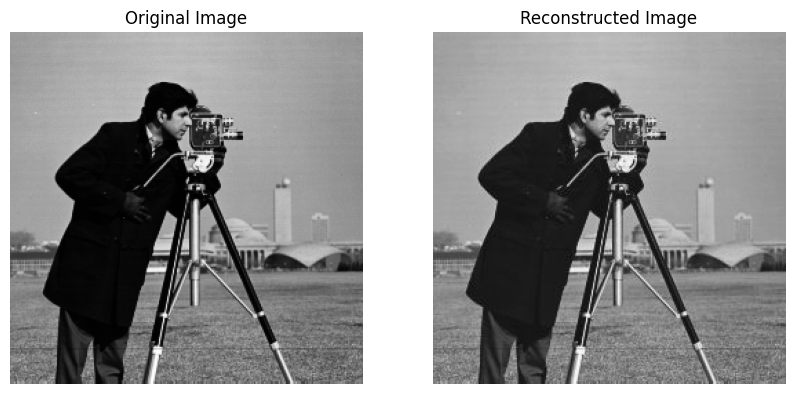
\includegraphics[width=1.0\linewidth]{images/im1q1.png}
        \caption{Provided sample file}
    \end{figure}}

    \begin{itemize}
        \item Percentage of zeroes : 74.942 \%
        \item Peak SNR (in dB)     : 35.7245 dB
    \end{itemize}



    \item Quality level 35
    {\begin{figure}[h]
        \centering
        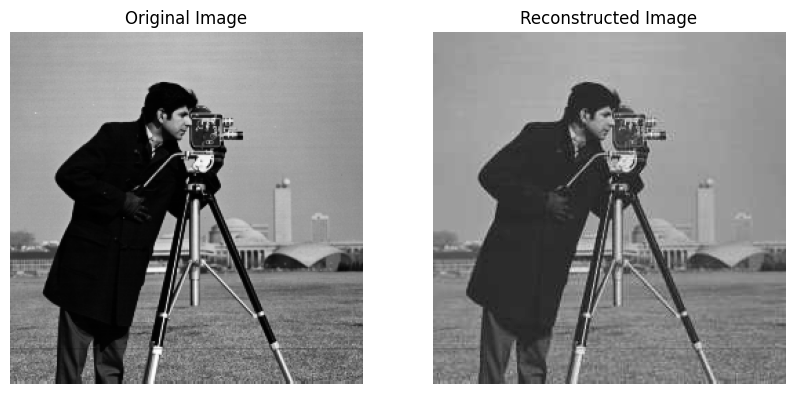
\includegraphics[width=1.0\linewidth]{images/im1q2.png}
        \caption{Provided sample file}
    \end{figure}}

    \begin{itemize}
        \item Percentage of zeroes : 88.275 \%
        \item Peak SNR (in dB)     : 30.3056 dB
    \end{itemize}


    \newpage



    \item Quality level 15
    {\begin{figure}[h]
        \centering
        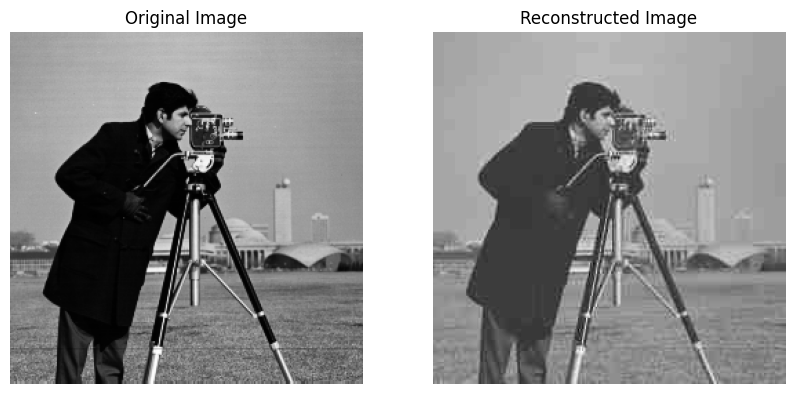
\includegraphics[width=1.0\linewidth]{images/im1q3.png}
        \caption{Provided sample file}
    \end{figure}}

    \begin{itemize}
        \item Percentage of zeroes : 93.348 \%
        \item Peak SNR (in dB)     : 27.536 dB
    \end{itemize}


\end{itemize}

\subsection{Image 02 : boat512} 

\begin{itemize}
    \item Quality level 80
    {\begin{figure}[h]
        \centering
        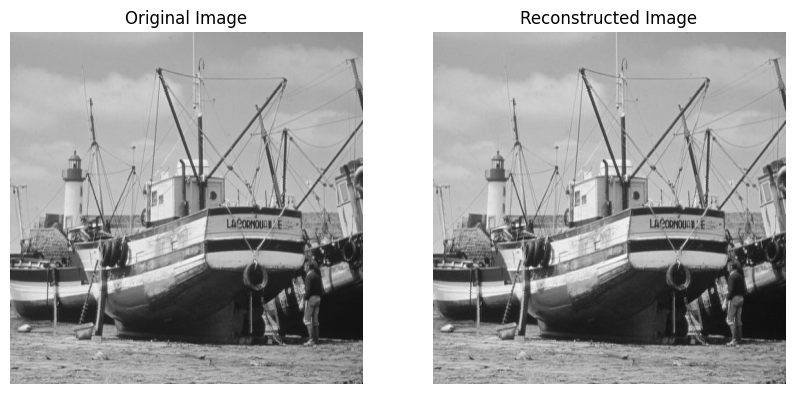
\includegraphics[width=1.0\linewidth]{images/im2q1.png}
        \caption{Provided sample file}
    \end{figure}}

    \begin{itemize}
        \item Percentage of zeroes : 78.343 \%
        \item Peak SNR (in dB)     : 38.0537 dB
    \end{itemize}



    \item Quality level 35
    {\begin{figure}[h]
        \centering
        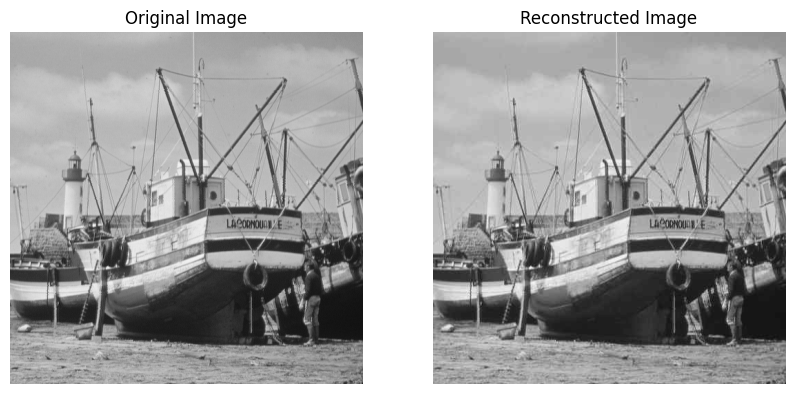
\includegraphics[width=1.0\linewidth]{images/im2q2.png}
        \caption{Provided sample file}
    \end{figure}}

    \begin{itemize}
        \item Percentage of zeroes : 89.334 \%
        \item Peak SNR (in dB)     : 29.9607 dB
    \end{itemize}

    \newpage



    \item Quality level 15
    {\begin{figure}[h]
        \centering
        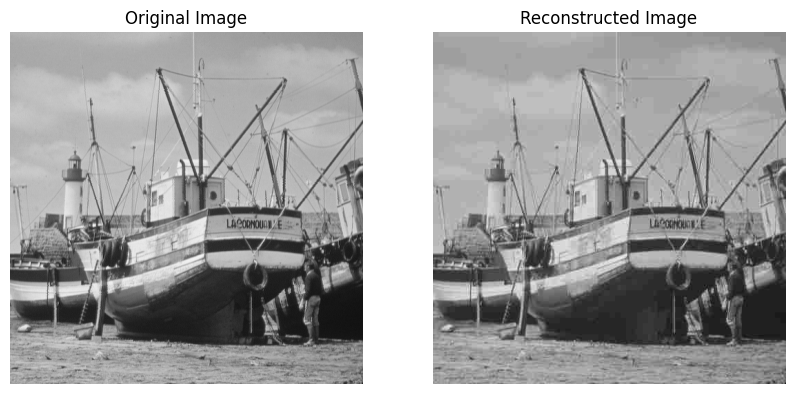
\includegraphics[width=1.0\linewidth]{images/im2q3.png}
        \caption{Provided sample file}
    \end{figure}}

    \begin{itemize}
        \item Percentage of zeroes : 93.820 \%
        \item Peak SNR (in dB)     : 60.1594 dB
    \end{itemize}

    
\end{itemize}


\subsection{Image 03 : peppers512} 

\begin{itemize}
    \item Quality level 80
    {\begin{figure}[h]
        \centering
        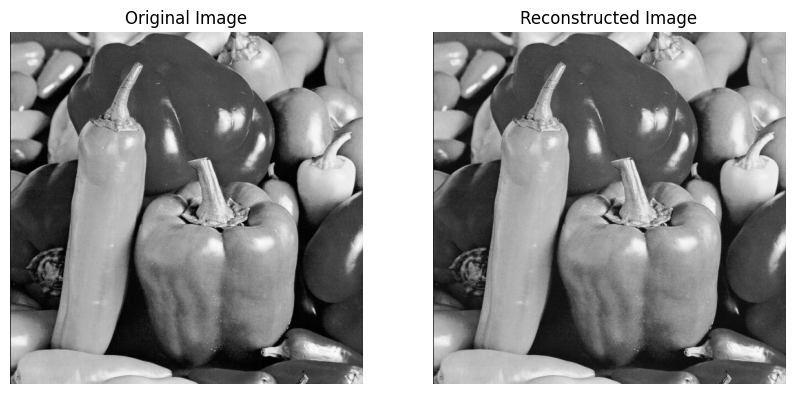
\includegraphics[width=1.0\linewidth]{images/im3q1.png}
        \caption{Provided sample file}
    \end{figure}}

    \begin{itemize}
        \item Percentage of zeroes : 79.283 \%
        \item Peak SNR (in dB)     : 36.9139 dB
    \end{itemize}



    \item Quality level 35
    {\begin{figure}[h]
        \centering
        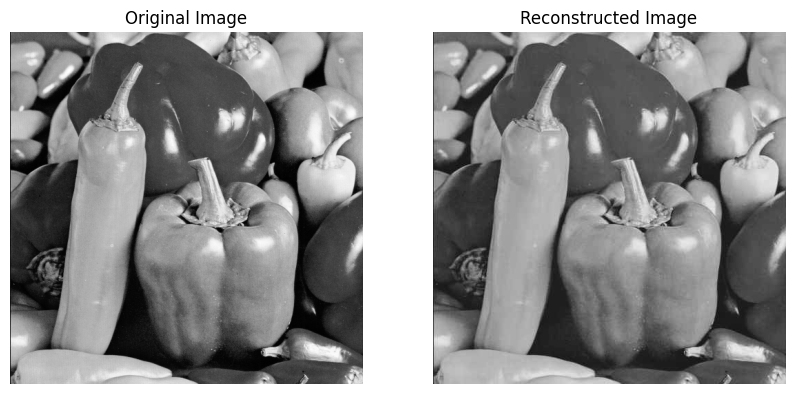
\includegraphics[width=1.0\linewidth]{images/im3q2.png}
        \caption{Provided sample file}
    \end{figure}}

    \begin{itemize}
        \item Percentage of zeroes : 91.356 \%
        \item Peak SNR (in dB)     : 33.9170 dB
    \end{itemize}

    \newpage



    \item Quality level 15
    {\begin{figure}[h]
        \centering
        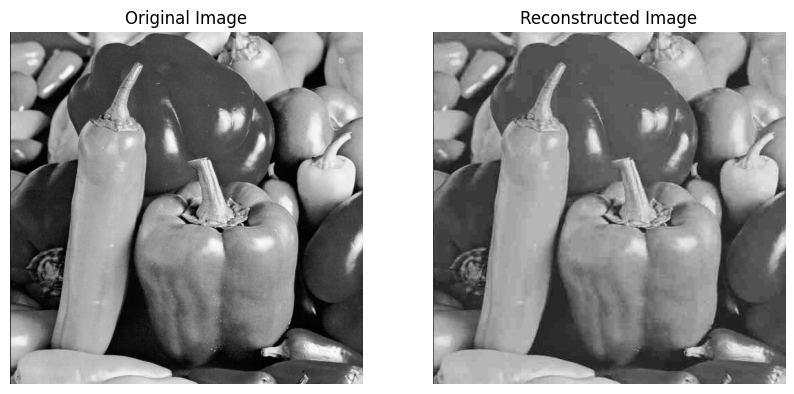
\includegraphics[width=1.0\linewidth]{images/im3q3.png}
        \caption{Provided sample file}
    \end{figure}}

    \begin{itemize}
        \item Percentage of zeroes : 94.886 \%
        \item Peak SNR (in dB)     : 31.5075 dB
    \end{itemize}

    
\end{itemize}


\subsection{Image 01 : Camera256} 

\begin{itemize}
    \item Quality level 80
    {\begin{figure}[h]
        \centering
        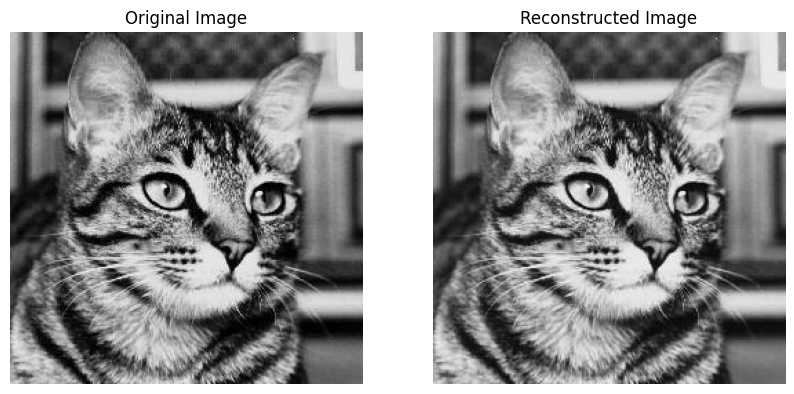
\includegraphics[width=1.0\linewidth]{images/im4q1.png}
        \caption{Provided sample file}
    \end{figure}}

    \begin{itemize}
        \item Percentage of zeroes : 67.567 \%
        \item Peak SNR (in dB)     : 40.7102 dB
    \end{itemize}



    \item Quality level 35
    {\begin{figure}[h]
        \centering
        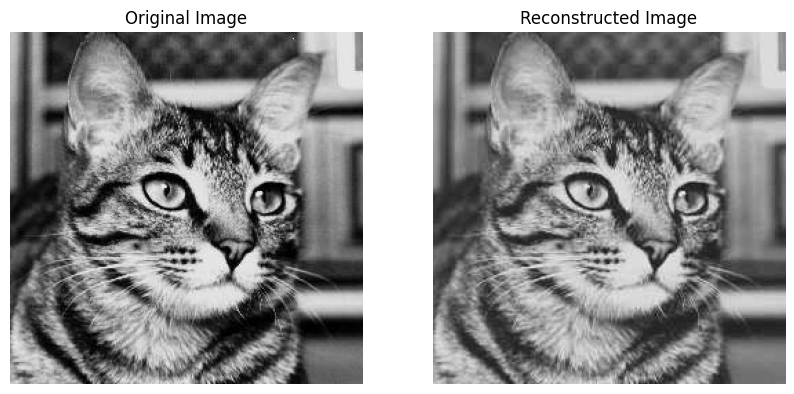
\includegraphics[width=1.0\linewidth]{images/im4q2.png}
        \caption{Provided sample file}
    \end{figure}}

    \begin{itemize}
        \item Percentage of zeroes : 82.170 \%
        \item Peak SNR (in dB)     : 28.4592 dB
    \end{itemize}

    \newpage


    \item Quality level 15
    {\begin{figure}[h]
        \centering
        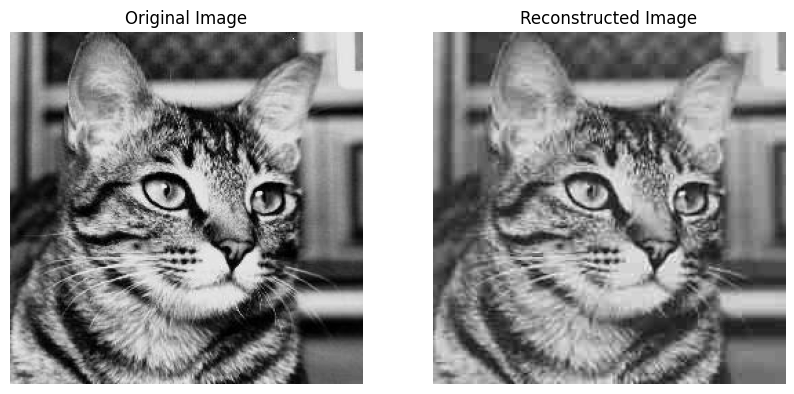
\includegraphics[width=1.0\linewidth]{images/im4q3.png}
        \caption{Provided sample file}
    \end{figure}}

    \begin{itemize}
        \item Percentage of zeroes : 89.554 \%
        \item Peak SNR (in dB)     : 25.7649 dB
    \end{itemize}

    
\end{itemize}


\section{Difficulty in Compression}


\section{References}

\begin{itemize}
    \item \href{https://numpy.org/doc/}{Numpy Documentation}
    \item \href{https://www.pearson.com/en-us/subject-catalog/p/discrete-time-signal-processing/P200000003226}{Preferred Text Book}
    % \item \href{ }{Github/EN3160_Assignment_01}
   
\end{itemize}

\section{Github Repository}

Following is the link to my Github repository for this assignment.\\

\href{https://github.com/Vgr20/EN3551_Assignment_02.git}{Github/EN3551\_Assignment\_02}


\newpage

\twocolumn
\section{Appendix}

\subsection{Extracting and Preparing the Data}

\lstset{style=mystyle}
\lstinputlisting[language=Octave]{code1.py}

\subsection{DCT and Quantization}

\lstset{style=mystyle}
\lstinputlisting[language=Octave]{code2.py}

\subsection{Coding Schemes}

\lstset{style=mystyle}
\lstinputlisting[language=Octave]{code3.py}

\subsection{Inverse DCT and re-construction}

\lstset{style=mystyle}
\lstinputlisting[language=Octave]{code4.py}

\subsection{Evaluation Metrics}

\lstset{style=mystyle}
\lstinputlisting[language=Octave]{code5.py}


\end{document}




%%%%%%%%%%%%%%%%%%%%%%%%%%%%%%%%%%%%%%%%%%%%%%%%%%%%%%%%%%%%%%%%%%%%%%%%%%%%%%%%%%%%%%%%%%%%%%%%%%%%%%%%%%%%%%%%%%%%%%%%%%%%%%%%%%%%%%%%%%%%%%%%%%%%%%%%%%%%%%%%%%%%%%%%%%

% {\begin{center}
% \begin{tabular}{ | m{1.85cm} | m{0.85cm}| m{0.85cm} | m{0.85cm} | m{0.85cm} | m{0.85cm} | } 
%  \hline
%  Objectives& Weight & Design 01 & Design 02 & Design 03 & Design 04 \\  
%  \hline\hline
%  Efficiency & 10 & 7 & 8 & 8 & 9 \\
%  \hline
%  Mobility & 10 & 7 & 9 & 8 & 8 \\
%  \hline
%  Easy Maintenance & 10 & 7 & 6 & 5 & 8 \\
%  \hline
%  Refilling accessibility & 5 & 3 & 3 & 2 & 4 \\
%  \hline
%  Durability & 5 & 2 & 3 & 3 & 2 \\
%  \hline
%  Manufacture cost & 5 & 3 & 3 & 2 & 3 \\
%  \hline
%  Overall Look & 5 & 2 & 3 & 5 & 2 \\
%  \hline
%  \hline
%  Total & 50 & 31 & 35 & 33 & 36 \\
%  \hline
 
% \end{tabular}
% \end{center}}

%%%%%%%%%%%%%%%%%%%%%%%%%%%%%%%%%%%%%%%%%%%%%%%%%%%%%%%%%%%%%%%%%%%%%%%%%%%%%%%%%%%%%%%%%%%%%%%%%%%%%%%%%%%%%%%%%%%%%%%%%%%%%%%%%%%%%%%%%%%%%%%%%%%%%%%%%%%%%%%%%%%%%%%%%%


% \begin{center}
% \begin{tabular}{ | m{2cm} | m{5cm}| m{2cm} | m{6cm} | } 

%  \hline
%  Part Name & Description & Supplier & Part Link\\  
%  \hline\hline
%  NE555P & 8-pin Precise timer & Texas Instruments & \href{https://www.lcsc.com/product-detail/Timers-Clock-Oscillators_Texas-Instruments-NE555P_C46749.html}{NE555p data sheet}\\
%  \hline
%  2N2222A & Generic npn transistor & Slkor & \href{https://www.lcsc.com/product-detail/Bipolar-Transistors-BJT_Slkor-SLKORMICRO-Elec-2N2222A_C5330385.html}{2N2222A data sheet}\\
%  \hline
%   LM7805 & Linear voltage Regulators & LRC & \href{https://www.lcsc.com/product-detail/Linear-Voltage-Regulators-LDO_LRC-LR7805_C2846986.html}{Lm7805 Data sheet}\\
%  \hline
%   HC sr501 & Passive IR sensor & HC & \href{https://www.lcsc.com/product-detail/Timers-Clock-Oscillators_Texas-Instruments-NE555P_C46749.html}{HC sr501 data sheet}\\
%  \hline
%   KNSCHA ZE11000UF & 1000uF Capacitor & KNSCHA & \href{https://www.lcsc.com/product-detail/Solid-Capacitors_KNSCHA-ZE11000UF35V119EC0014_C2992586.html}{Capacitor data sheet}\\
%  \hline
%   Resistors & Resistors with different values & Texas Instruments & \href{https://www.lcsc.com/search?q=resistors%20through%20hole}{Through hole resistors}\\
%  \hline
 
% \end{tabular}  
% \end{center}
%%%%%%%%%%%%%%%%%%%%%%%%%%%%%%%%%%%%%%%%%%%%%%%%%%%%%%%%%%%%%%%%%%%%%%%%%%%%%%%%%%%%%%%%%%%%%%%%%%%%%%%%%%%%%%%%%%%%%%%%%%%%%%%%%%%%%%%%%%%%%%%%%%%%%%%%%%%%%%%%%%%%%%%%%%